% THIS IS SIGPROC-SP.TEX - VERSION 3.1
% WORKS WITH V3.2SP OF ACM_PROC_ARTICLE-SP.CLS
% APRIL 2009
%
% It is an example file showing how to use the 'acm_proc_article-sp.cls' V3.2SP
% LaTeX2e document class file for Conference Proceedings submissions.
% ----------------------------------------------------------------------------------------------------------------
% This .tex file (and associated .cls V3.2SP) *DOES NOT* produce:
%       1) The Permission Statement
%       2) The Conference (location) Info information
%       3) The Copyright Line with ACM data
%       4) Page numbering
% ---------------------------------------------------------------------------------------------------------------
% It is an example which *does* use the .bib file (from which the .bbl file
% is produced).
% REMEMBER HOWEVER: After having produced the .bbl file,
% and prior to final submission,
% you need to 'insert'  your .bbl file into your source .tex file so as to provide
% ONE 'self-contained' source file.
%
% Questions regarding SIGS should be sent to
% Adrienne Griscti ---> griscti@acm.org
%
% Questions/suggestions regarding the guidelines, .tex and .cls files, etc. to
% Gerald Murray ---> murray@hq.acm.org
%
% For tracking purposes - this is V3.1SP - APRIL 2009

\documentclass{acm_proc_article-sp}

\usepackage{xspace}
\usepackage{color}
%\usepackage{hyphenation}
\hyphenation{Map-Reduce}

\newif\ifdraft
\drafttrue

\ifdraft
\newcommand{\terminology}[1]{ {\textcolor{red} {(Terminology used: \textbf{#1}) }}}
\newcommand{\jhanote}[1]{ {\textcolor{red} { ***shantenu: #1 }}}
\newcommand{\alnote}[1]{ {\textcolor{blue} { ***andreL: #1 }}}
\newcommand{\pnote}[1]{ {\textcolor{magenta} { ***pradeep: #1 }}}
\newcommand{\note}[1]{ {\textcolor{brown} { ***Note: #1 }}}
\else
\newcommand{\terminology}[1]{}
\newcommand{\alnote}[1]{}
\newcommand{\pnote}[1]{}
\newcommand{\jhanote}[1]{}
\newcommand{\note}[1]{}
\fi



\newcommand{\pilot}{Pilot\xspace}
\newcommand{\pilots}{Pilots\xspace}
\newcommand{\pilotjob}{Pilot-Job\xspace}
\newcommand{\pilotjobs}{Pilot-Jobs\xspace}
\newcommand{\pilotmapreduce}{PilotMapReduce\xspace}
\newcommand{\computeunit}{Compute Unit\xspace}
\newcommand{\computeunits}{Compute Units\xspace}
\newcommand{\cu}{CU\xspace}
\newcommand{\cus}{CUs\xspace}
\newcommand{\cs}{Compute Service\xspace}
\newcommand{\css}{Compute Services\xspace}
\newcommand{\pcs}{Pilot Compute Service\xspace}
\newcommand{\dataunit}{Data Unit\xspace}
\newcommand{\dataunits}{Data Unit\xspace}
\newcommand{\du}{DU\xspace}
\newcommand{\dus}{DUs\xspace}
\newcommand{\pilotdata}{Pilot-Data\xspace}
\newcommand{\pd}{PD\xspace}
\newcommand{\pds}{Pilot Data Service\xspace}
\newcommand{\pdss}{Pilot Data Services\xspace}
\newcommand{\su}{SU\xspace}
\newcommand{\sus}{SUs\xspace}
\newcommand{\schedulableunit}{Schedulable Unit\xspace}
\newcommand{\schedulableunits}{Schedulable Units\xspace}
\begin{document}

\title{An extensible Pilot-based MapReduce Implementation}

%
% You need the command \numberofauthors to handle the 'placement
% and alignment' of the authors beneath the title.
%
% For aesthetic reasons, we recommend 'three authors at a time'
% i.e. three 'name/affiliation blocks' be placed beneath the title.
%
% NOTE: You are NOT restricted in how many 'rows' of
% "name/affiliations" may appear. We just ask that you restrict
% the number of 'columns' to three.
%
% Because of the available 'opening page real-estate'
% we ask you to refrain from putting more than six authors
% (two rows with three columns) beneath the article title.
% More than six makes the first-page appear very cluttered indeed.
%
% Use the \alignauthor commands to handle the names
% and affiliations for an 'aesthetic maximum' of six authors.
% Add names, affiliations, addresses for
% the seventh etc. author(s) as the argument for the
% \additionalauthors command.
% These 'additional authors' will be output/set for you
% without further effort on your part as the last section in
% the body of your article BEFORE References or any Appendices.

\numberofauthors{3} %  in this sample file, there are a *total*
% of EIGHT authors. SIX appear on the 'first-page' (for formatting
% reasons) and the remaining two appear in the \additionalauthors section.
%
\author{
% You can go ahead and credit any number of authors here,
% e.g. one 'row of three' or two rows (consisting of one row of three
% and a second row of one, two or three).
%
% The command \alignauthor (no curly braces needed) should
% precede each author name, affiliation/snail-mail address and
% e-mail address. Additionally, tag each line of
% affiliation/address with \affaddr, and tag the
% e-mail address with \email.
%
\alignauthor Pradeep Kumar Mantha\\
       \affaddr{Center for Computation and Technology}\\
       \affaddr{Louisiana State University}\\
       \affaddr{216 Johnston}\\
       \affaddr{Baton Rouge, LA}
       \email{pmanth2@cct.lsu.edu}
\alignauthor Andre Luckow\\
       \affaddr{Center for Computation and Technology}\\
       \affaddr{Louisiana State University}\\
       \affaddr{216 Johnston}\\
       \affaddr{Baton Rouge, LA}
       \email{aluckow@cct.lsu.edu} 
\alignauthor Shantenu Jha\titlenote{Author for correspondence}\\
      \affaddr{Center for Autonomic Computing}\\
     \affaddr{Rutgers University}\\
      \affaddr{94 Brett Road}\\
      \affaddr{Piscataway, NJ}
     \email{shantenu.jha@rutgers.edu}
}
% There's nothing stopping you putting the seventh, eighth, etc.
% author on the opening page (as the 'third row') but we ask,
% for aesthetic reasons that you place these 'additional authors'
% in the \additional authors block, viz.
% \additionalauthors{Additional authors: John Smith (The Th{\o}rv{\"a}ld Group,
% email: {\texttt{jsmith@affiliation.org}}) and Julius P.~Kumquat
% (The Kumquat Consortium, email: {\texttt{jpkumquat@consortium.net}}).}
\date{30 July 1999}
% Just remember to make sure that the TOTAL number of authors
% is the number that will appear on the first page PLUS the
% number that will appear in the \additionalauthors section.

\maketitle
\begin{abstract}
In recent years, there has been a large increase in the size of computational
data which is widely distributed across different geographic locations. Timing and
cost-effective processing of these large-distributed datasets on distributed
computational resources requires effective management of data and compute
resources. Pilot-Jobs are successful in uptaking the distributed
infrastructures by compute intensive applications, but still there is a
necessity of an abstraction for data intensive applications to provide
coupling between data and compute units through a set of relationships.
Pilot-Data provides an abstraction for expressing and managing relationships
between data and/or compute units. The coupling of Pilot abstractions,
Pilot-Job and Pilot-Data, through SAGA Pilot API implementation, provides
flexibility to specify the relationship between compute and data units and
thus effective management of compute and data units across distributed
infrastructures. MapReduce is an effective programming model for processing
large distributed datasets. However, processing widely-distributed data sets
using traditional MapReduce setup configurations limits concurrent usage of
distributed infrastructure and depending on the type of workload aggregation,
overheads like huge data transfers or additional computation to combine
results are involved [weissmanns]. Most MapReduce implementations however,
tied to specific infrastructure. In this paper, we describe the design and
implementation of Pilot API based SAGA MapReduce (PMR), which is 
infrastructure
independent and extensible to multiple clusters. We validate and characterize
PMR by benchmarking it with Hadoop MapReduce using canonical word count
application. We present a PMR workflow to post-process data produced by deep
sequencing machines at widely-distributed geographic locations. The workflow
takes the output of the sequencing machines, performs short-read mapping using
BWA aligner, and removes duplicate reads. Our experiments show that it
provided a significantly improved throughput as it scaled to multiple
clusters, over traditionally distributed MapReduce~\cite{weissman-mr-11}.
\end{abstract}

% A category with the (minimum) three required fields
\category{D.1.2}{Software}{MapReduce}
%A category including the fourth, optional field follows...
\category{J.3}{Computer Applications}{Bioinformatics, Mapping}

% \terms{Design, Experimentation, Performance}

\keywords{Pilot-Jobs, Pilot-Data, Data-Intensive, MapReduce, Genome Sequence
Alignment, BWA, Human Genome, MapReduce, Distributed Computing, Simple API for
Grid Applications (SAGA)}% NOT required for Proceedings

\section{Introduction}

There are various challenges associated with data at extreme scales: which
have become a critical factor in many sciences disciplines, e.\,g.\ in the
areas of fusion energy (ITER), bioinformatics (metagenomics), climate (Earth
System Grid), and astronomy
(LSST)~\cite{Berriman:2011:AAS:2039359.2047483,Jha:2011fk}. The volumes of
data produced by these scientific applications are increasing rapidly driven
by advancing technologies (e.\,g.\ increasing compute capacity and higher
resolution sensors) and decreasing costs for computation, data acquisition and
storage~\cite{hey2009}. The number of scientific applications that either
currently utilize, or need to utilize large volumes of potentially distributed
data is immense. The challenges faced by these applications are
interoperability, efficiently managing compute tasks, and moving data to the
scheduled compute location, which is inevitable in case of programming models
like MapReduce.


But, processing huge amounts of data is a challenging tasks.
MapReduce~\cite{Dean:2004:MSD:1251254.1251264} as originally developed by
Google aims to address the big data problem by providing an easy-to-use
abstraction for parallel data processing. However, in many cases data is
highly distributed. While existing MapReduce perform very well on single
machines, they show severe limitations in highly distributed scenarios.


Pilot-Jobs have been notable in their ability to manage the compute units
across multiple high performance clusters, providing decoupling between
compute units and resource assignment, but there is also a need of an
abstraction to liberate applications/users from challenging requirement of
moving data to the scheduled compute location to execute it successfully.
Pilot-Data provides an abstraction for expressing and managing relationships
between data units and/or compute units. The coupling of abstractions,
Pilot-Jobs and Pilot-Data, provide a complete solution for data intensive
applications to utilize distributed cyber infrastructure effectively. The SAGA
Pilot-API is an implementation of P* model, and provides flexibility to manage
compute, data and relationships between them (affinities)~\cite{pstar-2012}.

MapReduce is an effective programming model for processing large datasets and
can be easily scaled across multiple clusters, involves execution of map
compute tasks, shuffling and moving the intermediate data to the reduce task
for successful execution~\cite{Dean:2004:MSD:1251254.1251264}. Most MapReduce 
implementations however, are tied to
specific infrastructure and are limited to a single cluster. When the source
data and computing platform distributed widely, the most efficient
architecture for processing data over the entire data set becomes non-trivial.
MapReduce setup configurations like Local MapReduce (LMR), Global
MapReduce (GMR) , Distributed MapReduce (DMR) were proposed to process the
distributed data, depending on the workload aggregation
scheme~\cite{weissman-mr-11}. In all these configurations, the huge factor
contributing towards time to solution is, time involved in transferring huge
amounts of data transfer either before the map phase or in shuffle phase.

By carefully analyzing the data movement patterns in MapReduce programming
model, we understood the importance of moving compute to data in the map
phase, and moving only required data to complete the reduce task in the
shuffle phase. These patterns and the limitations of MapReduce programming
model to utilize distributed cyber infrastructure motivated us, to use Pilot
abstractions for managing the map and reduce tasks and intermediate shuffle
data between them.

The key take-aways of this paper are:
\begin{itemize}
	\item MapReduce simplifies the construction of data-parallel applications
	\item Pilot-Abstraction enable the clean separation of resource management concerns and MapReduce.
	\item The Pilot/SAGA-based approach enables a maximum of portability, interoperability and code-reuse.
	\item Hadoop is designed for cluster/local environment, but not for a high degree of distribution.
	\item Future work: dynamic execution
\end{itemize}

In section II we talk about background-- Pilot API, Pilot-Job, Pilot-Data,
saga, SAGA previous implementation of MapReduce, Genome sequencing MapReduce
application. In section III, we discuss how Pilot abstractions, Pilot-Job and
Pilot-Data used to implement the architecture of MapReduce.,. In section IV we
discuss about the experiments.

\section{Related Work}

The MapReduce programming model~\cite{Dean:2004:MSD:1251254.1251264} and the
distributed file system (Google File System
(GFS)~\cite{Ghemawat:2003:GFS:1165389.945450} it is based on was originally
pioneered by Google. Apache Hadoop~\cite{hadoop} is an open source
implementation of MapReduce. Hadoop also includes an implementation of a
distributed file system -- the Hadoop File System
(HDFS)~\cite{Borthakur:2007fk}. In addition the Hadoop ecosystems includes
several other projects, such as HBase (a system also inspired by Google's
BigTable), Hive, Pig and Zookeeper.

Sphere

Twister/Iterative Map Reduce~\cite{Ekanayake:2010:TRI:1851476.1851593} is a 
MapReduce addressing particularly the requirement for supporting iterative 
MapReduce jobs. Twister allows the flexible composition of applications by 
specifying map and reduce tasks and the data flow between 
these tasks. 

Dryad

Twitter Storm

\section{Pilot Compute and Pilot Data}

Pilot-Jobs support effective distributed resource utilization, and are arguably one of the most widely-used distributed computing abstractions. 

\subsection{Pilot Abstractions for Compute and Data}

The abstraction of a {\emph Pilot-Job} generalizes the reoccurring concept of
utilizing a placeholder job as a container for a set of compute tasks;
instances of that placeholder job are commonly referred to as Pilot-Jobs or
pilots. The PJ provides applications (user) level control and management of
the set of allocated resources. Analogous to \pilotjobs, {\emph Pilot-Data}
provides late-binding capabilities for data by separating the allocation of
physical storage and application-level data units~\cite{pstar-2012}.

The Pilot-API exposes the core functionalities of a \pilot framework via a
unified interface providing a common API that can be used across multiple PJ
frameworks. The API provides three core classes: the
\texttt{PilotComputeService} for the management of Pilot-Jobs,
\texttt{PilotDataService} for the management of Pilot-Data and the
\texttt{ComputeDataService} for the management of \texttt{ComputeUnits} (CUs)
and \texttt{DataUnits} (DUs). A CU represents a primary self-containing piece
of work, while a DU represents a logical set for data~\cite{pstar-2012}.

\subsection{BigData: A Pilot-Data Implementation}
\begin{figure}[htbp]
	\centering
		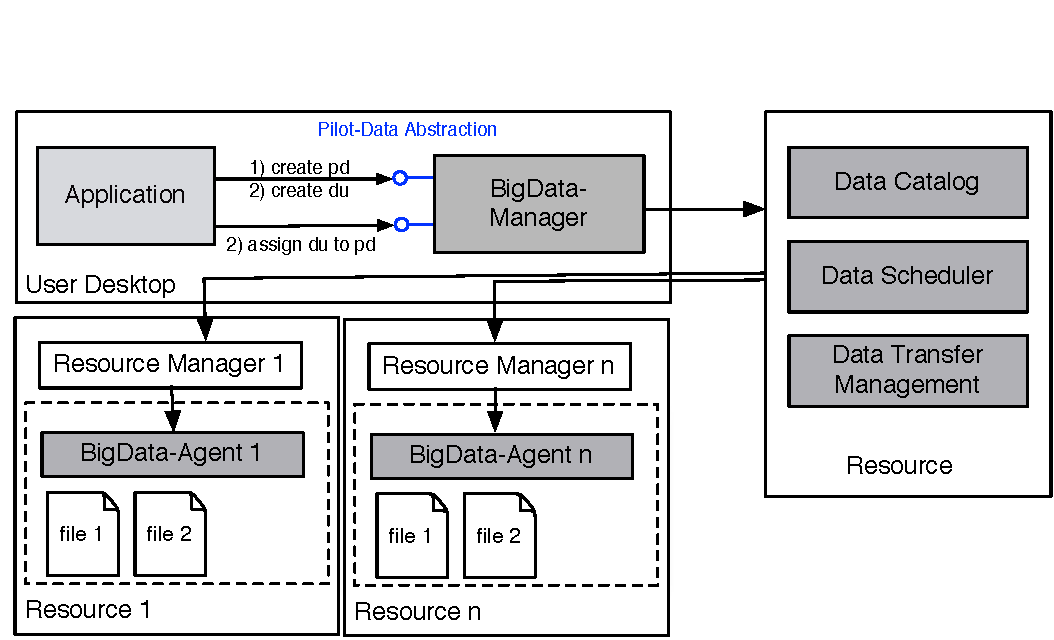
\includegraphics[width=0.47\textwidth]{figures/bigdata.pdf}
	\caption{BigData Architecture and Interactions}
	\label{fig:figures_bigdata}
\end{figure}

BigData (BD) is the SAGA-based prototype of the Pilot-Data abstraction.
BigData is based on BigJob~\cite{bigjob_web} -- a SAGA-based Pilot-Job
implementation. Figure~\ref{fig:figures_bigdata} gives an overview of the
architecture. The system consists similarly to BigJob of two components: the
BD-Manager and the BD-Agents deployed on the physical resources. The
coordination scheme used is again M/W with some intelligence that is located
de-centrally at the BD-Agent. As communication mechanism the SAGA Advert
Service is used, in a similar push/pull mode as for BJ.

The BD-Manager is responsible for (i) meta-data management, i.\,e.\ it
keeps track of the pilot stores that a pilot data object is associated
with, (ii) for scheduling data movements and data replications (taking
into account the application requirements defined via affinities), and
(iii) for managing data movements activities. For this purpose, it can rely
on external service, e.\,g.\ Globus Online for data transfer management.  
Similar to BigJob, an agent on each resource is used to manage the physical 
storage on a resource.  

A particular critical requirement for data-intensive application, is
the management of affinity between CUs and also between DUs and
DUs. The BD scheduler supports preliminary affinity-aware
scheduling: both BigJob and BigData are tightly integrated to
efficiently support compute- and data-related aspects of dynamic
execution.


\section{PilotMapReduce -- A Pilot-based MapReduce Implementation}
\alnote{We should only use PilotMapReduce to refer to our framework - SAGA does not need to be in the name and mentioned all the time}


{\emph \pilotmapreduce} provides a \pilot based implementation of the 
MapReduce programming model decoupling the core MapReduce framework from the 
actual management of the compute, data and network resources. By decoupling 
job scheduling and monitoring from the resource management, \pilotmapreduce 
can efficiently re-use the resource management and late-binding capabilities 
of BigJob and BigData.

PilotMapReduce exposes an easy-to-use interface which provides the complete
functionality needed by any MapReduce algorithm, while hiding the more complex
functionality, such as chunking of the input, sorting the intermediate
results, managing and coordinating the workers, etc. — these are generically
implemented by the framework.

\alnote{Can we put a code snipped in here somewhere? maybe a separate sub-section}

\pilotmapreduce uses the Pilot-API for managing map and reduce compute units
and for defining relationships between the intermediate data and reduce tasks
across distributed infrastructure. The SAGA MapReduce framework is responsible
for:

\begin{itemize} 
\item Chunking the input data, whether data is
local/distributed. The SAGA MapReduce framework uses SAGA Job package to
launch user defined chunk scripts on all the machines, which perform the
chunking of input data remotely.

 \item Launching Pilot-Jobs on all the clusters, where the data is located.
Once the Pilot-Job becomes active on that particular machine, it starts
executing map compute units on the local data. This avoids huge transfer of
input data before starting actual MapReduce which is in the case of
LMR~\cite{weissman-mr-11}

 \item ...still needs to be refined..................

 \item Collecting and grouping of partitioned and sorted intermediate data
output files related to a reduce. The framework prepares

 \item assigning the input data to the workers of the map step;

 \item handling the intermediate data files produced by the map step;

 \item Passing the location of the sorted output files to the workers of the
reduce step. \end{itemize}


 


\subsection{Previous SAGA-based MapReduce Implementations}

In~\cite{Sehgal:2011:UAI:1945091.1945329} we investigated the scale-out of an 
MapReduce application on different infrastructures. The utilization of Pilot 
abstractions has several advantages: (i) compute and data pilots allow an 
efficient decoupling of resource allocation and usage, i.\,e.\ the MapReduce 
master can efficiently schedule compute units containing mapper and reduce 
tasks; (ii) the co-location of data and compute units descriptively defined 
and are automatically handled by Pilot framework; This enables the 
applications to easily trade-off data transfers and available compute 
capacities.

\subsection{Architecture of Pilot-based SAGA MapReduce}

Figure~\ref{fig:figures_mapreduce-pilotdata} shows the architecture of the 
Pilot-based MapReduce framework. PilotMR utilizes Compute Pilots for managing the execution of mapper and reduce tasks, and Data Pilots for managing the flow of data, i.\,e.\ for transferring the input data to the compute tasks and for transferring the intermediate results between mapper and reduce tasks.

\begin{figure}[htbp]
	\centering
	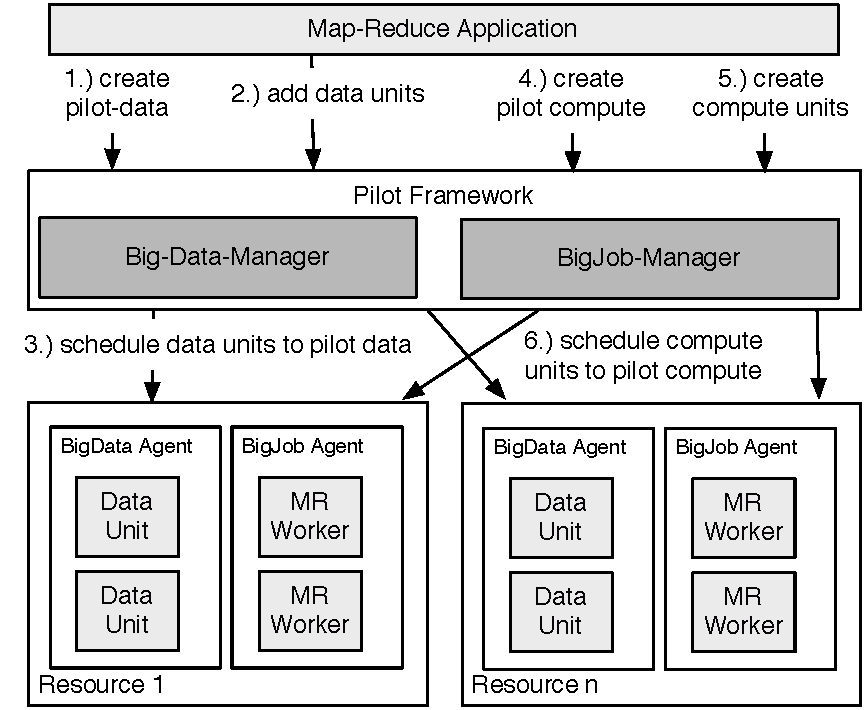
\includegraphics[width=0.4\textwidth]{figures/mapreduce-pilotdata.pdf}
	\caption{\textbf{Pilot-based MapReduce:} Each pilot (both compute and data 
	pilot) can be associated with an affinity label. The BigData and BigJob 
	Manager will ensure that CUs and DUs are placed with respect to these 
	requirements.}
	\label{fig:figures_mapreduce-pilotdata}
\end{figure}

Flow of an MapReduce application (assumption input data is pre-staged?):
\begin{enumerate}
	\item Start \pilotjobs on all resource.
	\item Execute \texttt{chunk} task via pilots
	\item Execute \texttt{mapper} tasks via pilots
	\item Move output data via Pilot Data
	\item Execute \texttt{reduce} tasks via pilots 
\end{enumerate}

Role of Pilot Data


\subsection{MapReduce Architectures for Distributed Data}

Motivate distributed data

There are three options for running MapReduce on distributed
data~\cite{weissman-mr-11}: (i) Local MapReduce, (ii) Global MapReduce and
(iii) Distributed MapReduce.


\section{MapReduce-Based Applications}


\subsection{Classifying MapReduce Applications}

Talk about different kinds of data aggregation

Iterative MapReduce


\subsection{WordCount}

basis for many machine learning use cases: classification, recommendation, etc.

\subsection{Genome sequencing duplicate read removal}

High-throughput genome sequencing techniques provided by Next Generation
Sequencing (NGS) platforms are changing biological sciences and biomedical
research. In this section we show how PilotMR can be used for a sequence
alignment application scenario.

\subsection{Discussion}

Contrast to Hadoop:
Pilot-MapReduce provides more flexibility and building block, e.g. flexible 
usage of sorting, more fine-grained control of data transfers etc.


%%%%%%%%%%%%%%%%%%%%%%%%%%%%%%%%%%%%%%%%%%%%%%%%%%%%%%%%%%%%%%%%%%%%%%%%%%%%

\section{Experiments and Results}
In this section we describe our specific experimental setups over FutureGrid platform:
FutureGrid: The FutureGrid is a collection of homogenous, highly distributed loosely-coupled clusters used for our study. In our experiments, we use India, Sierra and Hotel FutureGrid clusters. We use Hadoop 0.20.2 over FutureGrid machines for our study. In our experimental setups, to facilitate low overhead of the master processes(i.e., JobTracker and NameNode) given our workloads, we use 8 slaves nodes including master node. In all Hadoop MapReduce experiments, source data must be first pushed into HDFS before the MapReduce job starts. 
    We have two main experiments, involving WordCount and duplicate read removal Genome Sequencing application on different source data of text type. 

\subsection{Pilot MapReduce vs. Non-Pilot MapReduce}

1. Hadoop MapReduce (Hadoop MR) vs  Local-Pilot MapReduce (Local-PMR) vs Distibuted-Pilot MapReduce (distributed-PMR) using canonical word count application.


On FutureGrid, we used 8 nodes for Hadoop and Local-Pilot MapReduce on India cluster. In case of distributed-Pilot MapReduce, we use a total of 16 nodes in two widely separated clusters - 4 nodes on India, 4 nodes on Hotel. In case of Hadoop MR, data is already present on India cluster, but needs to be pushed into HDFS before Hadoop MapReduce is started. For local-PMR, data is already present on India cluster which is stored on a shared file system. For distributed-PMR, the total data is divided between India and Hotel cluster and is already present on shared file systems of each cluster. We set the number of reduces to 8 and chunk size is set to Hadoop default block size 128MB.

\subsection{Measuring Job completion time}
Hadoop MapReduce: Job completion time is measured as the MapReduce runtime in the main cluster, which involves time taken for MapReduce map, shuffle and reduce phases. To avoid overlap in calculating the map and shuffle phase times, we configure Hadoop MapReduce to start shuffle phase after MapReduce map phase is completed because with default configuration MapReduce shuffle phase might start before map phase completes. 

Local/Distributed-PMR: Job completion time is measured as the total runtime involved in chunking input data, MapReduce map, intermediate data transfer and reduce phases.

\subsection{Evaluation}
We ran 3 trails of each of experiment over the three types of MapReduce. We measured and plotted each component of the job completion time.

\begin{figure}[compMR]
	\centering
		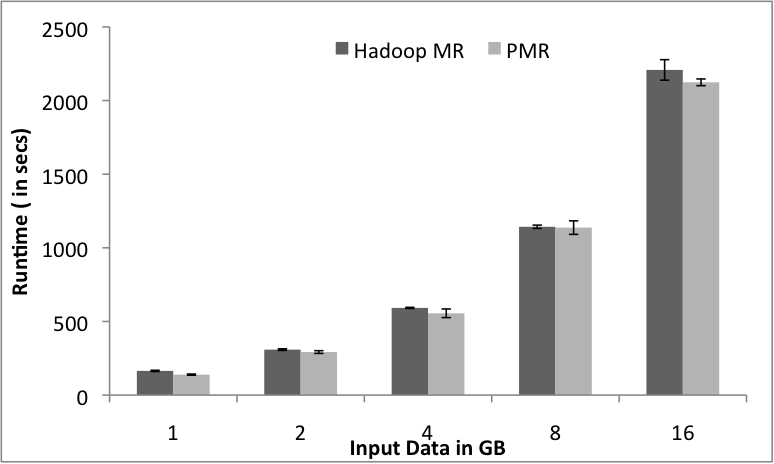
\includegraphics[width=0.47\textwidth]{figures/HMRvsL-PMRvsD-PMR.png}
	\caption{Pilot MapReduce vs Non-Pilot MapReduce}
	\label{fig:figures_compMR}
\end{figure}

The time to solution increased linearly as data size increased for Hadoop MapReduce, local-PMR, distributed-PMR. 
The Map phase time of Hadoop is 11.6% greater than Map phase time of Local-PMR because Hadoop MR involves preparing input splits and starting the map tasks, whereas in Pilot MapReduce, chunk time is considered seperatly and Map phase involves submitting of map compute units. The chunking time of distributed-Pilot MapReduce is less when compared to Local-PMR, since the data is halved and distributed to two machines. \pnote{ Andre::question::Hadoop uses logical splitting of files, where as PMR chunks the files physically, wiritng to disk, this is a performance bottlneck. Is acessing a single file, by many parallel subjobs cause problems?}. The shuffle phase is considered only in Hadoop MapReduce, where as the exchange is involved in Pilot MapReduce. The input to the reduce phase in all the three MapReduce increased linearly with input data. In local-PMR is < 1sec as the data is moved within cluster using SAGA file adaptor. In distributed PMR, the time to exchange data between India and Hotel also increased linearly with input data size. The Reduce phase is high for Pilot MR since the reduce compute units has to read intermediate data from the disk and write output data to the disk, where as in Hadoop MapReduce reduce phase, the intermediate data is available in memory and write the output to HDFS.


\begin{figure}[compMR_8GB]
	\centering
		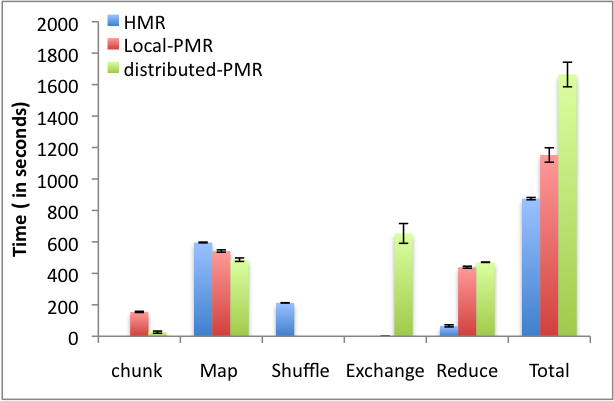
\includegraphics[width=0.47\textwidth]{figures/comparision_8gb.png}
	\caption{Wordcount on 8GB plain-text data}
	\label{fig:figures_compMR_8GB}
\end{figure}


Observed performance issues.			
1) File systems- hadoop performs better when nodes local data directory is used.. But performance degrades if shared storage is used. 			
2) when a single node is used to launch all workers, hadoop fails with lot of memory problems, whereas PMR successfully completed all tasks.			
reasons for this problem………..http://tech.backtype.com/the-dark-side-of-hadoop+J204		

(python)-bash-3.2$ hostname
i69
(python)-bash-3.2$ free -m
                  total          used       free     shared    buffers     cached
Mem:         24081       4524      19557          0        146       4128
-/+ buffers/cache:       248      23832
Swap:         2047          0       2047
	

         - varying input size (1GB, 2GB, 4GB, 8GB - experiments repeated for 3 times atleast..)

  



\subsection{Distributed MapReduce}

2. distributed PMR vs weissmann's implementation of  DMR using GS duplicate read removal application.

Weissmanns paper doesn't talk about low workload scheme applications where reduce output is still significantly large.. ( it talks about zero, high, balooning ).. so we have a model for these type of applications.

why weissmanns DMR is choosed?? LMR involves huge amount of initial data transfer. GMR need global filesystem across clusters, which is difficult to have, and latencies issues in moving files. So, DMR is a potential choice over LMR and GMR. 

DMR outperforms PMR if pilot-data doesn't transfer intermediate data concurrently. At the same time, if the concurrency  is not tuned properly, it might cause bandwidth problems.

------ So a experiment section needed to fine tune the concurrency between machines.. Again it depends on bandwidth and the machines use. need to perform experiments.

Infrastructure used - India, hotel, sierra futuregrid machines.. hotel is the fastest and sierra is slowest.

DMR implementation - use multiple Local PMR clusters and then combine their result with second round of Local PMR cluster. ( India, sierra, hotel) machines are used.
DMR tts = max ( tts of LMR on india, tts of LMR  on sierrra, tts of LMR  on hotel ) + max (reduce data transfer from india->hotel, reduce data transfer from sierra->hotel) + ( combined LMR on hotel ).. why hotel?? because the runtime on hotel is less.  

PMR tts = max( map  on india, map on  sierrra, map on hotel) + max( exchange of intermediate data between all machines(n) ( n * n-1 concurrent exchanges)) + max ( reduce phase on  india, reduce on  sierrra, reduce on hotel)

--- experiments done for local PMR on each individual cluster.. once time taken to trasnfer intermediate data between machines is obtained.. then tts for PMR can be caluculated and compared to DMR.

\subsection{Pilot MapReduce and Hadoop}


\section{Conclusions and Future Work}


Extending BigData: Access data through BigData abstraction.

BigData \& Realtime


%
% The following two commands are all you need in the
% initial runs of your .tex file to
% produce the bibliography for the citations in your paper.
\bibliographystyle{abbrv}
\bibliography{pilotjob,saga,saga-related,mrbib}  % sigproc.bib is the name of the Bibliography in this case
% You must have a proper ".bib" file
%  and remember to run:
% latex bibtex latex latex
% to resolve all references
%
% ACM needs 'a single self-contained file'!
%

cite p* paper,
cite weissmann
cite moore's law
cite script used to convert fastq to qseq
cite reference paper used to implement duplicate removal application.


\subsection*{Acknowledgments}
grants, funding, jhkim for providing data sets.

\end{document}
